\section{Multi-arm Bandits}
\subsection{Exercise 2.1}
\subsubsection*{Q}
In \(e\)-greedy action selection, for the case of two actions and \(e\) = 0.5, what is the probability that the greedy action is selected?

\subsubsection*{A}
Greedy action selected with \(p\) = 0.5
$
\hfill \blacksquare
$

\subsection{Exercise 2.2}
\subsubsection*{Q}
Bandit example Consider a k-armed bandit problem with k = 4 actions, denoted 1, 2, 3, and 4. Consider applying to this problem a bandit algorithm using \(e\)-greedy action selection, sample-average action-value estimates, and initial estimates of \(Q_1(a)\) = 0, for all \(a\). Suppose the initial sequence of actions and rewards is $A_1 = 1, R_1 = 1, A_2 = 2, R_2 = 1, A_3 = 2, R_3 = 2, A_4 = 2, R_4 = 2, A_5 = 3, R_5 = 0$. On some of these time steps the \(e\) case may have occurred, causing an action to be selected at random. On which time steps did this definitely occur? On which time steps could this possibly have occurred?

\subsubsection*{A}
\begin{table}[h!]
	\begin{tabular}{lllllll}
		\hline
		Timestep & \(Q_1\) & \(Q_2\) & \(Q_3\) & \(Q_4\) & Greedy action at timestep & Action selected \\  \hline
		0        & 0    & 0    & 0    & 0    & -                         & \(A_1\)     \\        \hline
		1        & 1    & 0    & 0    & 0    & \(A_1\)                      & \(A_2\)      \\       \hline
		2        & 1    & 1    & 0    & 0    & \(A_1/A_2\)                 & \(A_2\)      \\       \hline
		3        & 1    & 1.5  & 0    & 0    & \(A_2\)                      & \(A_2\)     \\        \hline
		4        & 1    & 1.66 & 0    & 0    & \(A_2\)                      & \(A_5\)    \\         \hline
		5        & 1    & 1.66 & 0    & 0    & \(A_2\)                      & end       \\       \hline
	\end{tabular}
	\label{table: ex2.2}
	\caption{Greedy actions at each timestep of a 4-armed bandit problem}
\end{table}
\begin{itemize}
	\item Action selection at timesteps 0, 1 and 4 are random as they are not reward maximising - see Table \ref{table: ex2.2}.
	\item Action selection at timestep 2 could be random as \(A_1\) is also reward maximising - see Table \ref{table: ex2.2}.
\end{itemize}
$
\hfill \blacksquare
$

\subsection{Exercise 2.3}
\subsubsection*{Q}
In the comparison shown in Figure \ref{fig:chapter2_2}, which method will perform best in the long run in terms of cumulative reward and probability of selecting the best action? How much better will it be? Express your answer quantitatively.

\subsubsection*{A}
In the limit of \(t \rightarrow \infty\), both non-zero \(e\)-greedy policies will learn the optimal action abd value function \(q*\). The policy with \(e\) = 0.01 will select the optimal action 10x more regularly than the policy with \(e\) = 0.1.
$
\hfill \blacksquare
$

\subsection{Exercise 2.4}
\subsubsection*{Q}
If the step-size parameters, \(\alpha_n\), are not constant, then the estimate \(Q_n\) is a weighted average of previously received rewards with a weighting different from that given by (2.6). What is the weighting on each prior reward for the general case, analogous to (2.6), in terms of the sequence of step-size parameters?.

\subsubsection*{A}
For a n-dependent \(\alpha\) we have:
\begin{align}
	Q_{n+1} &= Q_n +\alpha_n \left[R_n - Q_n\right] \nonumber \\
	&= \alpha_n R_n + (1-\alpha_n) Q_n\nonumber \\
	&= \alpha_n R_n + (1-\alpha_n) \left[Q_{n-1} + \alpha_{n-1} \left[R_{n-1} - Q_{n-1} \right]\right]\nonumber \\
	&= \alpha_n R_n + \alpha_{n-1} R_{n-1} - \alpha_n \alpha_{n-1} R_{n-1} + (1-\alpha_n)(1-\alpha_{n-1}) Q_{n-1} \nonumber \\
	&= \vdots \nonumber \\
	&= \sum_{i}^{n} \alpha_n R_n - R_{n-1} \prod_{i}^{n} \alpha_n + Q_{1} \prod_{i}^{n}(1-\alpha_n) \\
\end{align}
$
\hfill \blacksquare
$

\subsection{Exercise 2.5}
\subsubsection*{Q}
Design and conduct an experiment to demonstrate the difficulties that sample-average methods have for nonstationary problems. Use a modified version of the 10-armed testbed in which all the \(q_*(a)\) start out equal and then take independent random walks (say by adding a normally distributed increment with mean 0 and standard deviation 0.01 to all the \(q_*(a)\)  on each step). Prepare plots like Figure 2.2 for an action-value method using sample averages, incrementally computed, and another action-value method using a constant step-size parameter, \(\alpha\) = 0.1. Use \(\alpha\) = 0.1 and longer runs, say of 10,000 steps.

\subsubsection*{A}
\ProgrammingExercise
\begin{figure}[h!]
	\centering
	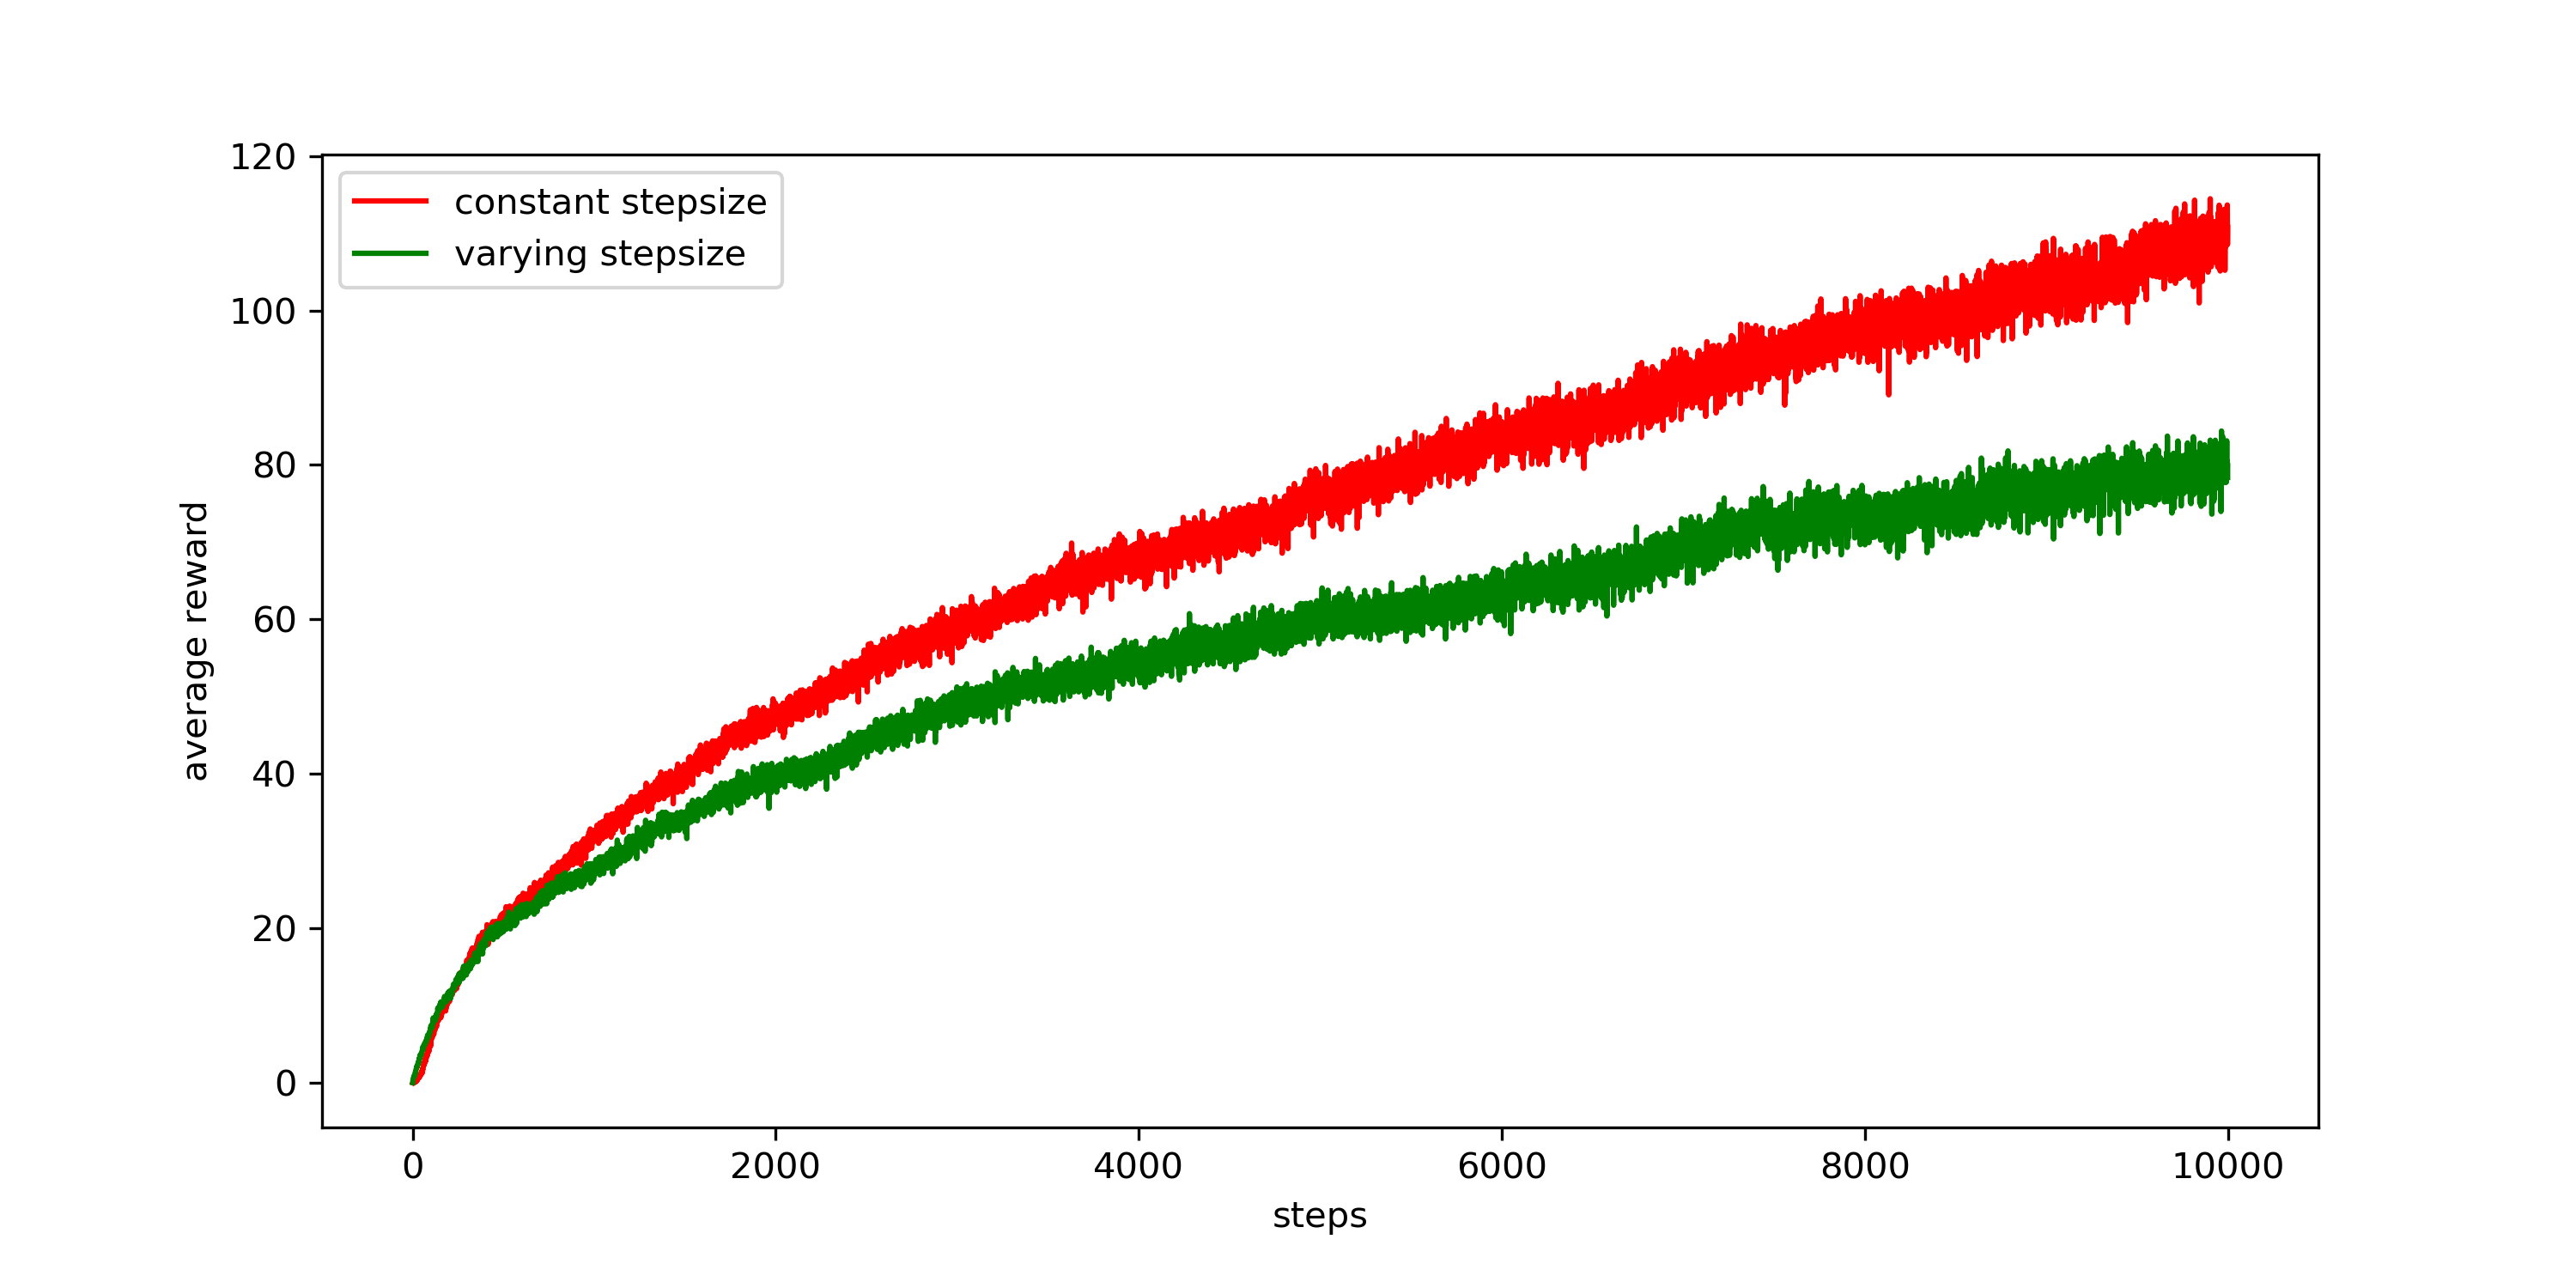
\includegraphics[width=\textwidth]{/ex2.5}
	\caption{Stationary versus varying stepsize \(alpha\) in a 10-armed bandit problem. We see that the constant stepsize parameter (exponential decay) performs better than the varying stepsize parameter as we place more weight on the recently observed (moving) values.}
	\label{fig:ex2.5}
\end{figure}
$
\hfill \blacksquare
$

\subsection{Exercise 2.6}
\begin{figure}[h!]
	\centering
	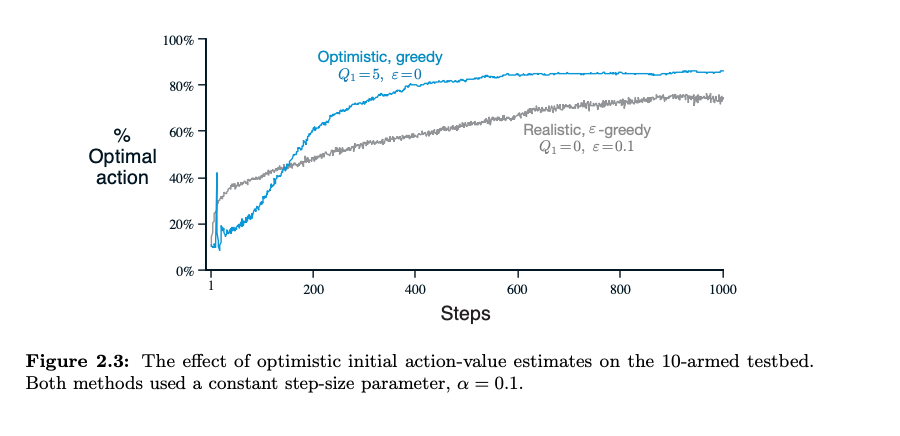
\includegraphics[width=\textwidth]{/chapter2_3}
	\caption{}
	\label{fig:chapter2_3}
\end{figure}

\subsubsection*{Q}
\textit{Mysterious Spikes}: The results shown in Figure 2.3 should be quite reliable because they are averages over 2000 individual, randomly chosen 10-armed bandit tasks. Why, then, are there oscillations and spikes in the early part of the curve for the optimistic
method? In other words, what might make this method perform particularly better or worse, on average, on particular early steps?

\subsubsection*{A}
The optimistic greedy policy with explore on every initial step as all value estimates are greater than their true value. It is possible, therefore, that it randomly selects the optimal action and then immediately forgets it in favour of yet-to-be-explored actions. This explains the spike at timestep \(\approx 10\).
$
\hfill \blacksquare
$

\subsection{Exercise 2.7}
\subsubsection*{Q}
Unbiased Constant-Step-Size Trick In most of this chapter we have used sample averages to estimate action values because sample averages do not produce the initial bias that constant step sizes do (see the analysis leading to (2.6)). However, sample averages are not a completely satisfactory solution because they may perform poorly on nonstationary problems. Is it possible to avoid the bias of constant step sizes while retaining their advantages on nonstationary problems? One way is to use a step size of
\begin{equation}
	\beta_n = \alpha / \bar{o_n}
\end{equation}

to process the \(n\)th reward for a particular action, where \(\alpha\) > 0 is a conventional constant step size, and ¯on is a trace of one that starts at 0:
\begin{equation}
	\bar{o_n} = \bar{o_{n-1}} + \alpha(1 - \bar{o_{n-1}}), for n > 0 and \bar{o_0} = 0.
\end{equation}

Carry out an analysis like that in (2.6) to show that Qn is an exponential recency-weighted
average without initial bias.

\subsubsection*{A}
If we recall our answer for Exercise 2.4 for varying stepsize, we see that \(Q_1\) is weighted by \(w = \prod_{i=1}^{\infty} (1 - \alpha_i)\). When \(i\) = 1, \(\beta_n\) = \(\alpha\), thus \(w \rightarrow 0 \forall i\) and \(Q_1\) no longer affects our estimate of \(Q_{n+1}\).
$
\hfill \blacksquare
$

\subsection{Exercise 2.8}
\subsubsection*{Q}
\textit{UCB Spikes} In Figure \ref{fig:chapter2_2} the UCB algorithm shows a distinct spike in performance on the 11th step. Why is this? Note that for your answer to be fully satisfactory it must explain both why the reward increases on the 11th step and why it decreases on the subsequent steps. Hint: If c = 1, then the spike is less prominent.

\subsubsection*{A}
After 10 timesteps the UCB algorithm has explored all 10 actions as, until they are selected, their upper confidence bound is infinite (as \(N_t(a)\) = 0) as so it guarenteed to be selected once in the first 10 actions. At this point the agent has one sample to assess the expected value of each arm and the same confidence/uncertainty in each action. With c < 0 it is likely to pick the action with highest return from first sample, which will likely give it an similarly large reward, creating the spike. Now, the upper confidence bound for that action will decrease and the agent will select another, less valuable action, causing the decrease in performance at the next timestep.
$
\hfill \blacksquare
$

\subsection{Exercise 2.9}
\subsubsection*{Q}
Show that in the case of two actions, the soft-max distribution is the same as that given by the logistic, or sigmoid, function often used in statistics and artificial neural networks.

\subsubsection*{A}
Soft-max distribution is defined as:
\begin{equation}
	Pr{A_t = a} \approx \frac{e^{H_t(a)}}{\sum_{b=1}^{k} e^{H_t(b)}} \approx \pi_t(a)
\end{equation}

For two actions \(1\) and \(2\) this becomes:

\begin{align}
	A_t  &= \frac{e^{H_t(1)}}{e^{H_t(1) + e^{H_t(2)}}}  \\
	&= \frac{e^{H_t(1)}}{e^{H_t(1)}}{(1 + \frac{e^{H_t(2)}}{e^{H_t(1)}}}  \\
	&= \frac{1}{e^{H_t(1)}(1 + e^{-x}}  \\
\end{align}
i.e. the sigmoid function with $x = H_t(1) - H_t(2)$.
$
\hfill \blacksquare
$

\subsection{Exercise 2.10}
\subsubsection*{Q}
Suppose you face a 2-armed bandit task whose true action values change randomly from time step to time step. Specifically, suppose that, for any time step, the true values of actions 1 and 2 are respectively 10 and 20 with probability 0.5 (case A), and 90 and 80 with probability 0.5 (case B). If you are not able to tell which case you face at any step, what is the best expected reward you can achieve and how should you behave to achieve it? Now suppose that on each step you are told whether you are facing case A or case B (although you still don’t know the true action values). This is an associative search task. What is the best expected reward you can achieve in this task, and how should you behave to achieve it?

\subsubsection*{A}
Part 1): If we do not know whether we are in task A or B we could decide pick the same action each time to maximise expected reward. Selecting either action 1 or action 2 every time would provide an expected reward of 50. Picking actions randomly would also provide an expected reward of 50 in this example.
Part 2): If we know we are in task A or B we can learn the optimal action for each (A(a) = 2 and B(a) = 1). Doing so would provide us a higher expected reward than the non-contextual case of 55.
$
\hfill \blacksquare
$